\documentclass[10pt,oneside]{article}
\usepackage[T1]{fontenc}
\usepackage[utf8]{inputenc}
%\DeclareUnicodeCharacter{00A0}{ }
\usepackage[adobe-utopia]{mathdesign}

\usepackage{amsmath}
\usepackage[francais]{babel}
\usepackage[dvips]{graphicx}
%\usepackage{here}
\usepackage{framed}
\usepackage[normalem]{ulem}
\usepackage{fancyhdr}
\usepackage{titlesec}
\usepackage{vmargin}

\usepackage{amsmath}
\usepackage{ifthen}
\usepackage{multirow}
\usepackage{multicol} % Portions de texte en colonnes

%\usepackage{xltxtra} % Logo XeLaTeX
%\usepackage{pst-solides3d}
\usepackage{color}
%\usepackage{colortbl}
\usepackage{titletoc} % Pour la mise en forme de la table des matières

%\usepackage[crop=off]{auto-pst-pdf}
%\usepackage{bclogo}


%\usepackage{longtable}
%\usepackage{flafter}%floatants après la référence
%\usepackage{pst-solides3d}
%\usepackage{pstricks}
%\usepackage{minitoc}
%\setcounter{minitocdepth}{4}
%\usepackage{draftcopy}% "Brouillon"
%\usepackage{floatflt}
%\usepackage{psfrag}
%\usepackage{listings} % Permet d'insérer du code de programmation
%\usepackage{lmodern}
%\usepackage[adobe-utopia,uppercase=upright,greeklowercase=upright]{mathdesign}
%\usepackage{minionpro}
%\usepackage{pifont}
%\usepackage{amssymb}
%\usepackage[francais]{varioref}

\setmarginsrb{1.5cm}{1cm}{1cm}{1.5cm}{1cm}{1cm}{1cm}{1cm}

\definecolor{gris25}{gray}{0.75}
\definecolor{bleu}{RGB}{18,33,98}
\definecolor{bleuf}{RGB}{42,94,171}
\definecolor{bleuc}{RGB}{231,239,247}
\definecolor{rougef}{RGB}{185,18,27}
\definecolor{rougec}{RGB}{255,230,231}
\definecolor{vertf}{RGB}{103,126,82}
\definecolor{vertc}{RGB}{220,255,191}
\definecolor{violetf}{RGB}{112,48,160}
\definecolor{violetc}{RGB}{230,224,236}
\definecolor{jaunec}{RGB}{220,255,191}

\usepackage[%
    pdftitle={SLCI - DS3},
    pdfauthor={Xavier Pessoles},
    colorlinks=true,
    linkcolor=blue,
    citecolor=magenta]{hyperref}



% \makeatletter \let\ps@plain\ps@empty \makeatother
%% DEBUT DU DOCUMENT
%% =================
\sloppy
\hyphenpenalty 10000

\newcommand{\Pointilles}[1][3]{%
\multido{}{#1}{\makebox[\linewidth]{\dotfill}\\[\parskip]
}}

\begin{document}


\newboolean{prof}
\setboolean{prof}{false}
%------------- En tetes et Pieds de Pages ------------
\pagestyle{fancy}
\renewcommand{\headrulewidth}{0.2pt}

\fancyhead{}
\fancyhead[L]{PTSI -- Sciences Industrielles pour l'Ingénieur}
\fancyhead[R]{Lycée Jules Haag -- Besançon}


\renewcommand{\footrulewidth}{0.2pt}
\fancyfoot[C]{\bfseries \thepage}
\fancyfoot[L]{2010 -- 2011}
\ifthenelse{\boolean{prof}}{%
\fancyfoot[R]{DS 3 -- SLCI -- Éléments de correction}
}{%
\fancyfoot[R]{DS 3 -- SLCI -- Éléments de correction}
}

%\fancyfoot[RO]{Version du \today}
% \fancyfoot[LE]{Version du \today}
% \fancyfoot[RO]{\textcolor{gris25}{Version rapporteurs}}
% \fancyfoot[LE]{\textcolor{gris25}{Version rapporteurs}}
% \fancyfoot[R]{\textcolor{gris25}{Version rapporteurs}}
% ----------------------------------------------------



\vspace{1cm}

\begin{center}
 \huge\textsc{Devoir Surveillé 3 -- Système de freinage de l'Airbus A318}

\vspace{1cm}

 \large\textsc{\'Eléments de correction}
\end{center}

\vspace{1cm}


\noindent\rule{\linewidth}{.2pt}
\begin{center}
\large\textbf{CI : 1} \textit{AF : Fonctionnalités, architecture et structure
des systèmes pluri techniques}

 \large\textbf{CI : 5} \textit{Communication technique : schémas et géométrie
des pièces}

 \large\textbf{CI : 7} \textit{SLCI : Comportement et modélisation des systèmes
automatiques. Identification }

 \large\textbf{CI : 8} \textit{Seq : Commande et comportement des systèmes à
événements discrets (Combinatoire et Séquentiel)}

\end{center}
\noindent\rule{\linewidth}{.2pt}



\section{Présentation du système}

\section{Description fonctionnelle du système de freinage}

\paragraph{}
\textit{Compléter à partir des explications précédentes et du SADT A-0, le SADT de niveau A0.}
\begin{center}
 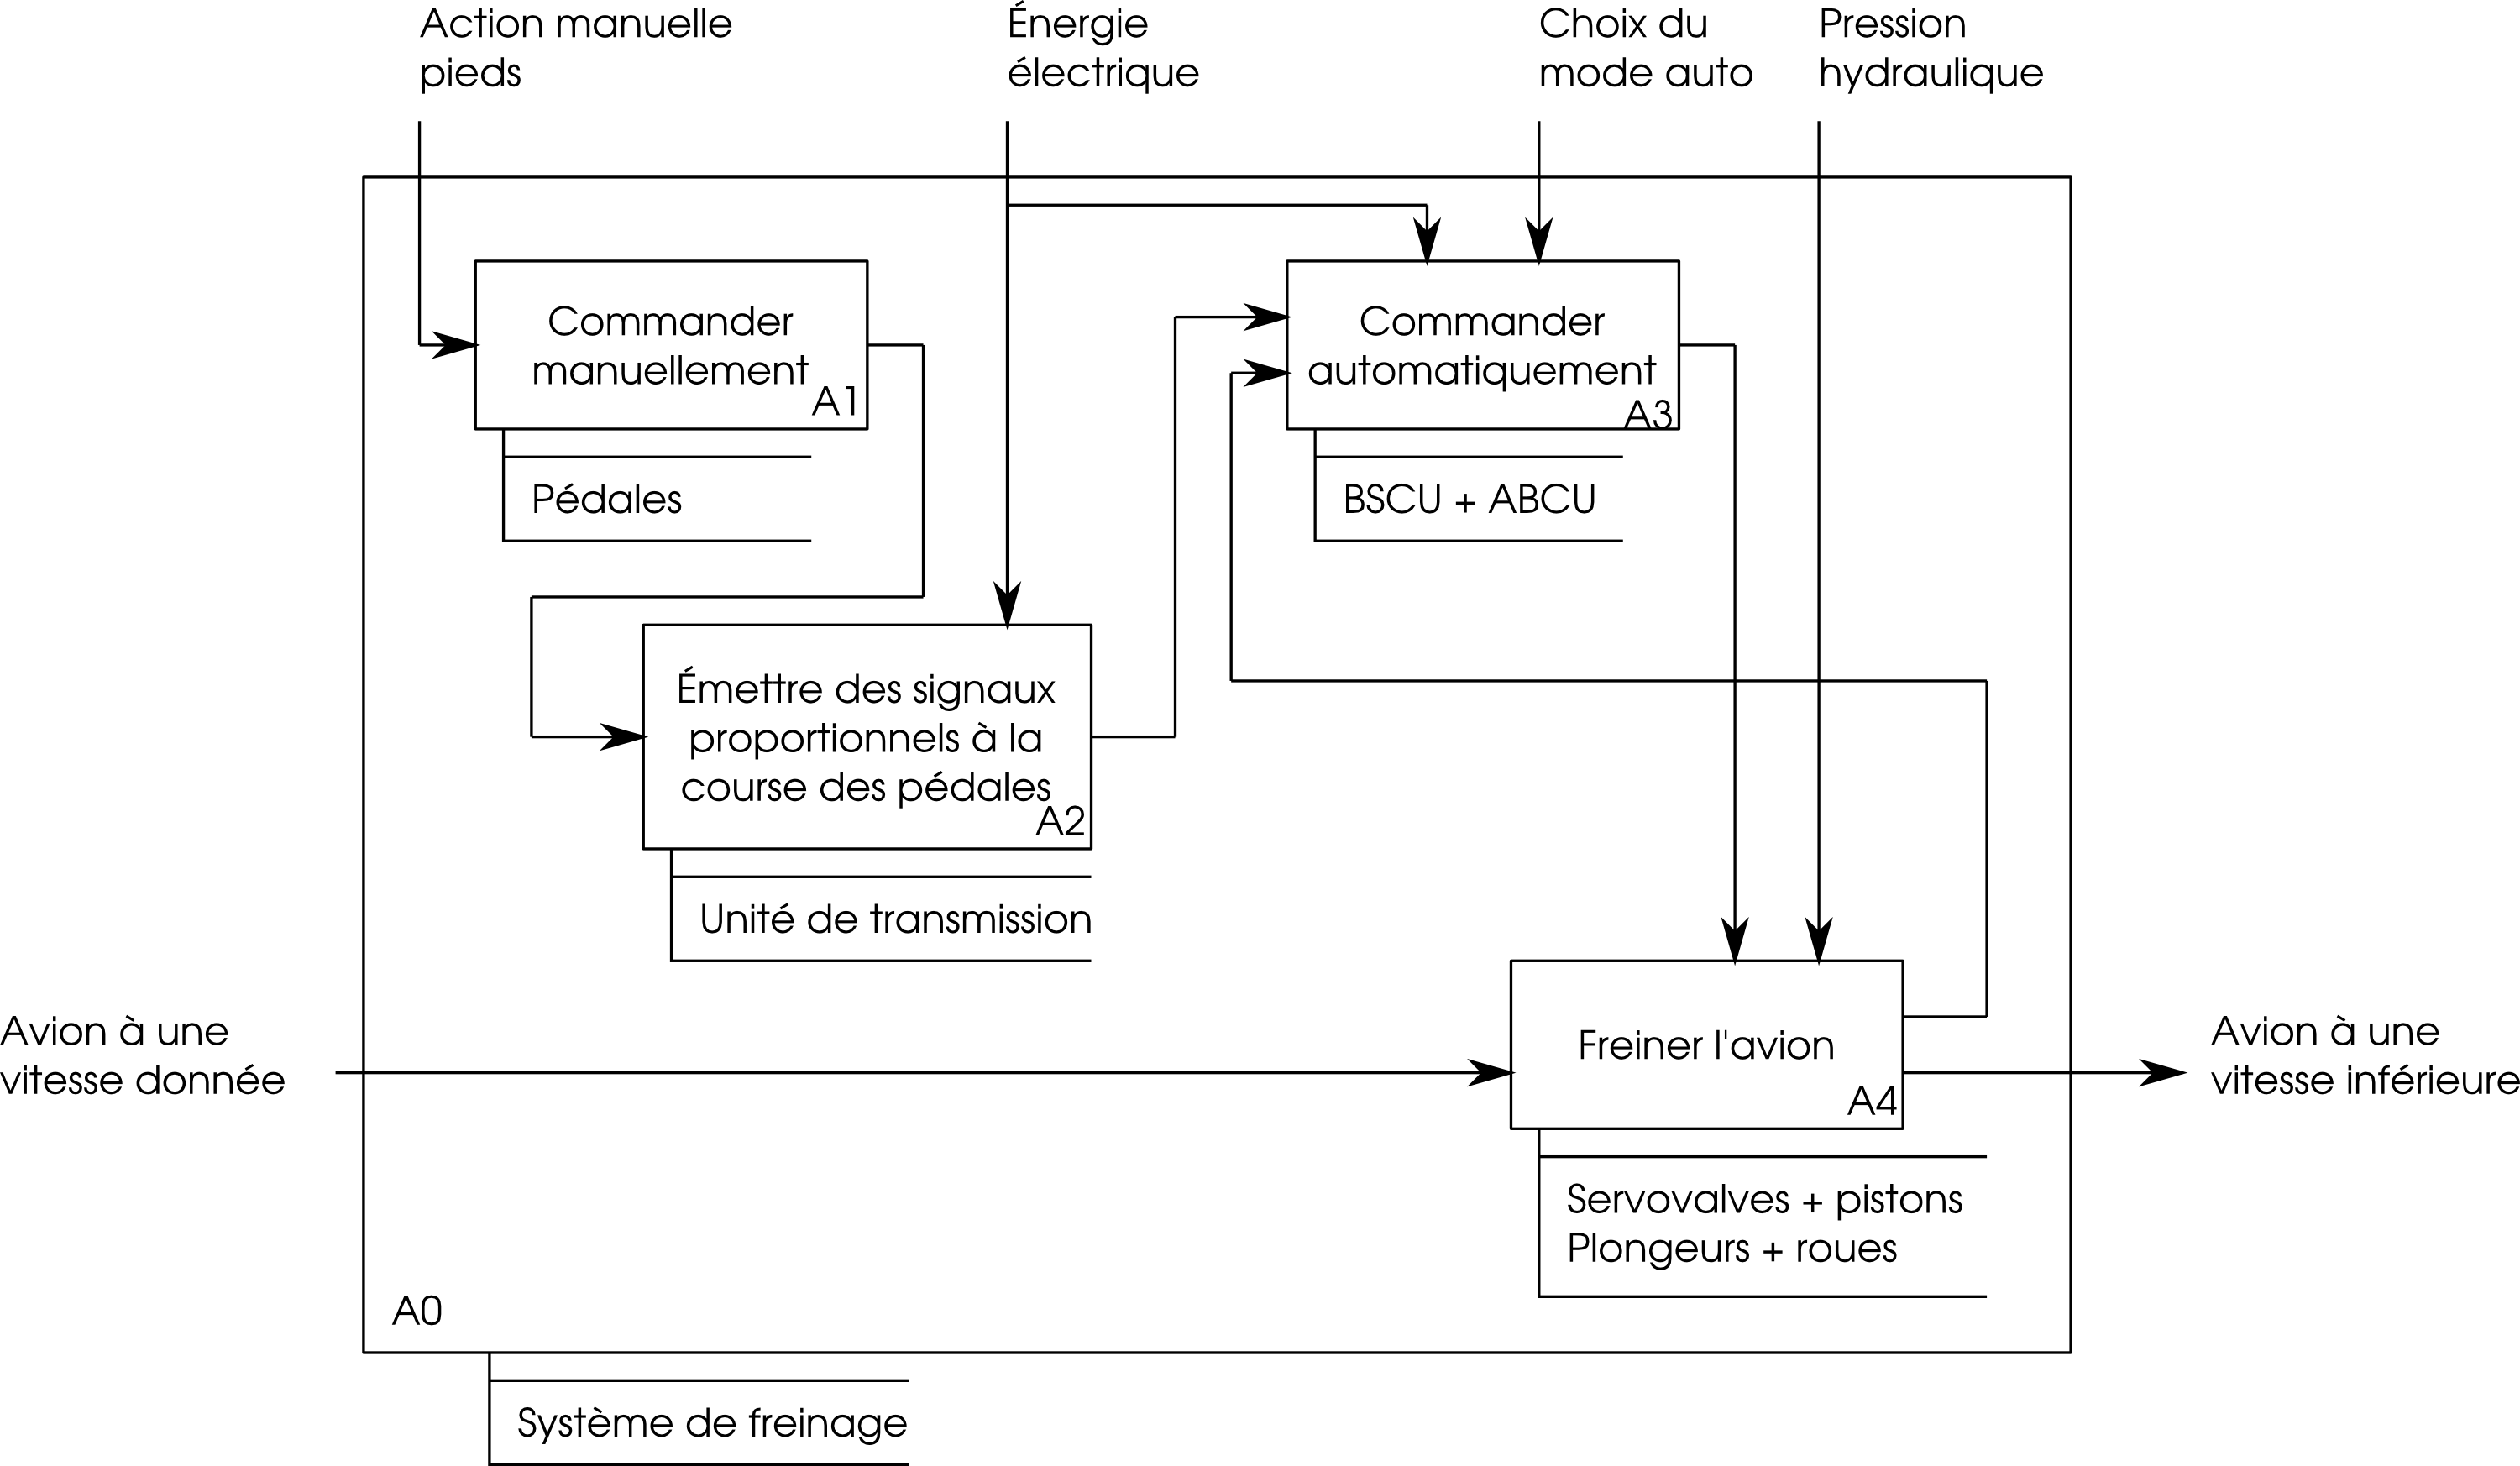
\includegraphics[width=.8\textwidth]{png/SADT}
\end{center}

\paragraph{}
\textit{Réaliser un schéma-bloc fonctionnel de l'asservissement en décélération à partir des
indications ci-dessus. On prendra $a_c(t)$ comme entrée et $a(t)$ comme sortie.}

\begin{center}
 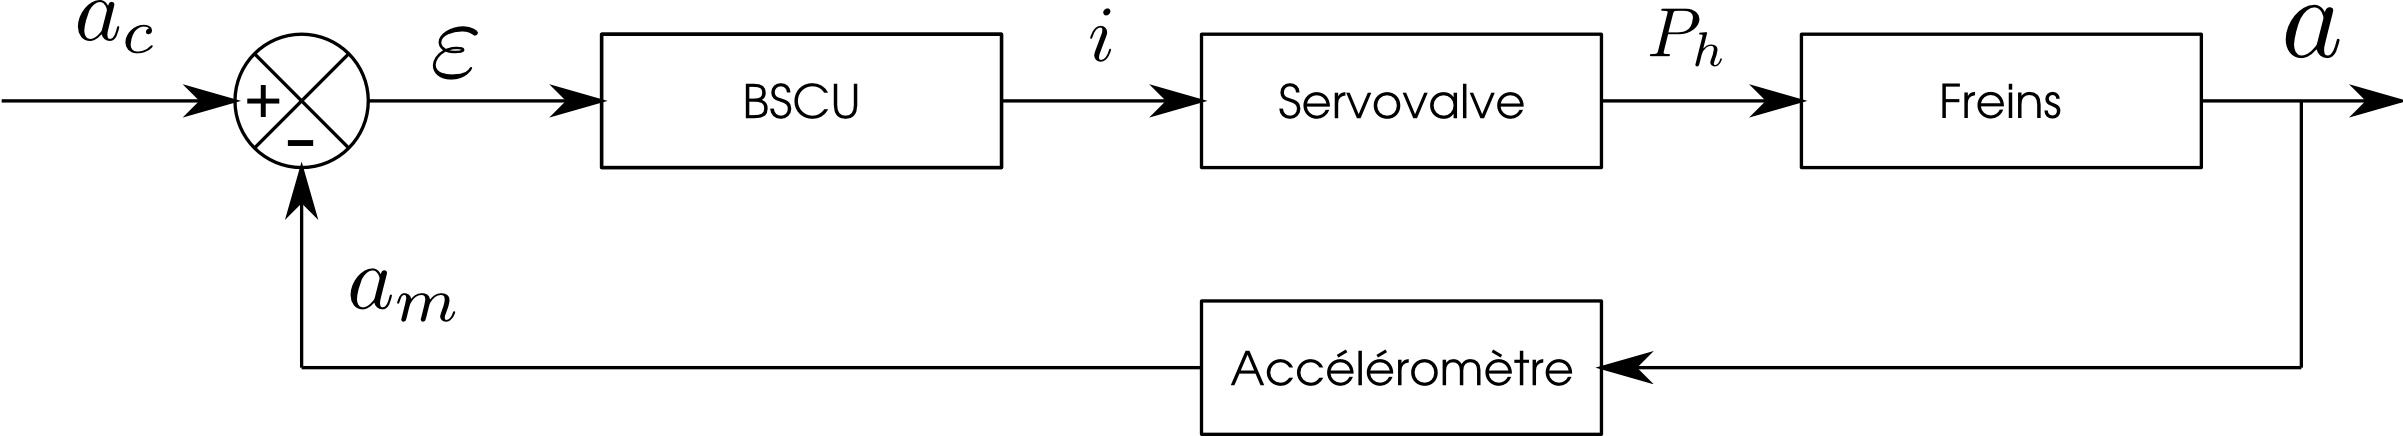
\includegraphics[width=.8\textwidth]{png/blocs}
\end{center}

\section{Modélisation du système de freinage}

\subsection{Modélisation de la servo-valve}

\paragraph{}
\textit{Que peut-on dire de cette caractéristique sur tout le domaine de variation de $i(t)$ ? Sachant
que $\theta$ est très petit (varie autour de 0), on utilise la relation suivante $\theta(t)=K_1i(t)$.
 Déterminer la valeur de $K_1$ à partir de la courbe.}

Cette courbe est non linéaire sur tout le domaine de variation de $i$. Comme
$\theta$ est très petit, on peut linéariser la courbe au voisinage de 0. La
valeur $K_1$ correspond donc à la pente  de la courbe. En conséquence,
$K_1=1\;rad\cdot A^{-1}$. 

\paragraph{}
\textit{Calculer la fonction de transfert $H_t(p)=\dfrac{Z(p)}{\Delta P(p)}$ 
où $Z(p)$ et $\Delta P(p)$ sont les transformées de Laplace de $z(t)$ et 
$\Delta P(t)$ en précisant l'hypothèse retenue.}

En se plaçant dans les conditions de Heaviside, on peut transformer l'équation
dans le domaine de Laplace. On a donc : 
$$
m_t p^2 Z(p) = -2k_t Z(p) + 2 S_t \Delta P(p) - pc_t Z(p)
$$

Ainsi, 

$$
H_t(p)=\dfrac{Z(p)}{\Delta P(p)} = \dfrac{2S_t}{m_tp^2+c_tp+2k_t}
$$

\paragraph{}
\textit{Mettre cette fonction de transfert sous forme canonique et donner son
ordre.}

En factorisant par $2k_t$ on obtient : 
$$
H_t(p)= \dfrac{\dfrac{S_t}{k_t}}{1+\dfrac{c_t}{2k_t}p+\dfrac{m_t}{2k_t}p^2}
$$

\paragraph{}
\textit{\`A partir de toutes les informations précédentes (modélisation armature, buse/palette,
tiroir...), compléter le schéma-bloc de la servo-valve donné dans le document réponse, en précisant les
fonctions de transfert de chaque bloc (utiliser les notations algébriques).}

On utilise les équation suivantes : 

$$
\theta(t)=K_1 i(t) \Leftrightarrow \Theta(p)=K_1 I(p)
$$

$$
\Delta S(t) = K_2 \theta (t) \Leftrightarrow  \Delta S(p) = K_2 \Theta (p)
$$

$$
\Delta P(t) = K_3 \Delta S(t) \Leftrightarrow  \Delta P(p) = K_3 \Delta S(p) 
$$

$$
P_h(t)=K_4 z(t) \Leftrightarrow   P_h(p)=K_4 Z(p) 
$$

On en déduit ainsi le schéma bloc suivant :
\begin{center}
 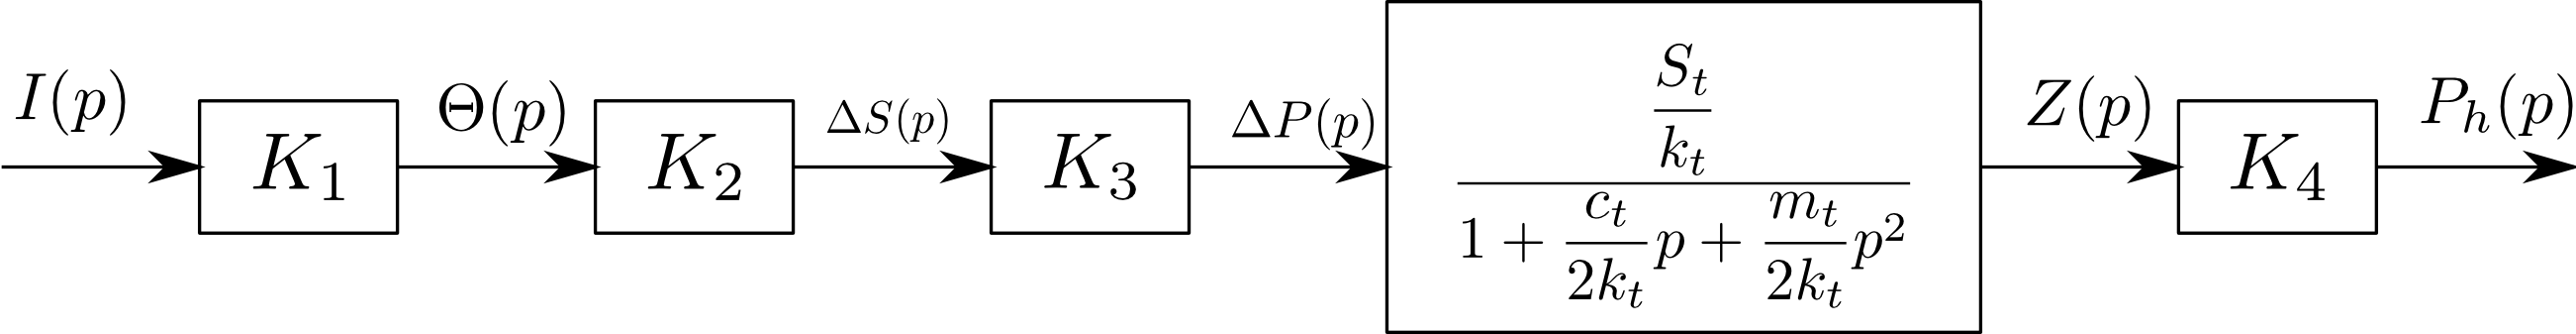
\includegraphics[width=.8\textwidth]{png/blocs2}
\end{center}

\paragraph{}
\textit{En déduire la fonction de transfert $S_v(p)=\dfrac{P_h(p)}{I(p)}$ de la
servo-valve.}

On en déduit directement : 
$$
S_v(p)=\dfrac{P_h(p)}{I(p)} = \dfrac{K_1 K_2 K_3 K_4
\dfrac{S_t}{k_t}}{1+\dfrac{c_t}{2k_t}+\dfrac{m_t}{2k_t}p^2}
$$

\paragraph{}
\textit{Montrer qu'elle peut se mettre sous la forme d'un système du second ordre :}
$$
S_v(p)=\dfrac{P_h(p)}{I(p)}=\dfrac{K_{sv}}{1+\dfrac{2\xi p}{\omega_0}+\dfrac{p^2}{\omega_0^2}}
$$
\textit{où on donnera les expressions littérales de $K_{sv}$, $\xi$ et
$\omega_0$.}

Par identification, on déduit de la question précédente : 
$$
K_{SV} = K_1 K_2 K_3 K_4
\dfrac{S_t}{k_t}
$$

$$
\omega_0 = \sqrt{\dfrac{2k_t}{m_t}}
$$

$$
\xi = \dfrac{c_t}{2\sqrt{2k_t m_t}}
$$
\paragraph{}
\textit{A quelle valeur de $\xi$ correspond cette spécification ?}
Pour ne pas avoir de dépassement, il est nécessaire que $\xi \geq 1$. Le
système est le plus rapide lorsque $\xi=1$.

\paragraph{}
\textit{Démontrer que cette condition ne peut être satisfaite que si
$k_t=\dfrac{c_t^2}{8m_t}$.}

$$
\xi = 1 \Leftrightarrow  c_t = 2\sqrt{2k_t m_t} \Leftrightarrow  k_t =
\dfrac{c_t^2}{8 m_t}
$$

\paragraph{}
\textit{Montrer alors que la fonction de transfert de la servo-valve peut se mettre sous la forme :}
$$
S_v(p)=\dfrac{P_h (p)}{I(p)}=\dfrac{K_{sv}}{\left( 1+T_{sv} p\right)^2 }
$$
\textit{on donnera l'expression littérale de $T_{sv}$.}

Lorsque $\xi=1$, le discriminant du dénominateur de la fonction
$S_v(p)$ est nul. En conséquence ce dénominateur possède une racine double. En
utilisant la formulation proposée, cette racine est égale à
$\dfrac{-1}{T_{sv}}$. En développant la fonction proposée, on peut donc
identifier $T_sv$ :
$$
\left( 1+T_{sv} p\right)^2  = 1+\dfrac{2
p}{\omega_0}+\dfrac{p^2}{\omega_0^2}  \Leftrightarrow 1 + 2 T_{sv} p +T_{sv}^2
p^2 = 1+\dfrac{2
p}{\omega_0}+\dfrac{p^2}{\omega_0^2}   
$$

On a donc : 
$$
T_{sv}=\dfrac{1}{\omega_0} = \sqrt{\dfrac{m_t}{2k_t}} = \sqrt{\dfrac{m_t}{2
\dfrac{c_t^2}{8 m_t}}} = 2\dfrac{m_t}{c_t}
$$

\paragraph{}
\textit{Déterminer la réponse indicielle $P_h(t)$ pour une entrée échelon de valeur $i(t)=i_0 u(t)$.}

On soumet le système à une entre échelon. En conséquence, on a : 
$$
I(p)=\dfrac{i_0}{p}
$$

On a alors :
$$
P_h(p)=\dfrac{i_0}{p}\dfrac{K_{sv}}{\left(1+T_{sv}p\right)^2}
$$

En réalisant la décomposition en éléments simples, on a : 
$$
P_h(p)=\dfrac{\alpha}{p}+\dfrac{\beta}{1+T_{sv}p}+\dfrac{\gamma}{\left(1+T_{sv}
p\right)^2}
$$

En calculant $P_h(p)p$ et en posant $p=0$, on obtient $\alpha = K_{sv}i_0$.

En calculant $P_h(p)\left(1+T_{sv} p\right)^2$ et en posant
$p=-\dfrac{1}{T_{sv}}$, on obtient $\alpha = K_{sv}i_0$. On obtient alors
$\gamma = - K_{sv} T_{sv} i_0$.

Enfin, en calculant $\lim\limits_{p\to +\infty} p P_h(p)$ on obtient $\beta =
-K_{sv} T_{sv} i_0$.

Au final, on obtient : 
$$
P_h(p) = K_{sv} i_0 \left( \dfrac{1}{p} - \dfrac{T_{sv}}{1+T_{sv}p} -
\dfrac{T_{sv}}{\left(1+T_{sv}p\right)^2} \right) 
=
K_{sv} i_0
\left( 
\dfrac{1}{p}
-\dfrac{1}{\dfrac{1}{T_{sv}}+p}
-\dfrac{\dfrac{1}{T_{sv}}}{\left(\dfrac{1}{T_{sv}}+p\right)^2}
\right) 
$$


En repassant dans le domaine temporel, on obtient :
$$
P_h(t) = K_{sv} i_0 \left( 
1-e^{-\dfrac{-t}{T_{sv}}}
-\dfrac{t}{T_{sv}}e^{-\dfrac{-t}{T_{sv}}}
\right) u(t)
$$
\paragraph{}
Recueil des meilleures blagues, les auteurs se reconnaîtront :
\begin{itemize}
 \item Monsieur, ne nous prenez pas pour des débiles, est-ce que vous avez déjà
vu un logarithme et une exponentielle dans un café ?
\item Que doit faire un proffesseur (NDLR les fautes ont été restituées telles
quelles) de mathématiques avant d'aller au soleil ?
\item À une fête $i$ va voir 1 et lui dit «Aller, on va dans danser ?»
\item Qu'est-ce qu'un ours polaire ?
\item $x^2$ et $\sqrt{x}$ sont sur un bateau, $\sqrt{x}$ tombe à l'eau, qui
est-ce qui reste ?
\end{itemize}

\subsection{Modélisation de l'accéléromètre}

\subsection*{Principe de l’accéléromètre}

\paragraph{}
\textit{Déterminer les transformées de Laplace des expressions (1) à (5).}

On obtient directement : 
$$
\varepsilon(p)=X_1(p)-X_2(p)
$$

$$
A(p)=p^2 X_1(p)
$$

$$
m_a p^2 X_2(p)=c_a \left( pX_1(p) - pX_2(p)\right)+k_a\left( X_1(p)
-X_2(p) \right)
$$

$$
U_a(p)=K_p \epsilon(p)
$$

$$
A_m(p)=K_{CAN} U_a(p)
$$
\paragraph{}
\textit{En déduire les transmittances $G_i$ du schéma bloc.}
On a : 
$$
G_1 = \dfrac{X_1(p)}{A(p)}=\dfrac{1}{p^2}
$$

D'après la troisième relation, on a :

$$
X_2(p)\left( m_a p^2 +c_a p + k_a \right) = X_1(p) \left( c_a p + k_a  \right)
$$
 et donc 
$$
G_2 = \dfrac{X_2(p)}{X_1(p)} = \dfrac{c_a p + k_a}{m_a p^2 +c_a p + k_a}
$$

$$
G_3 = \dfrac{U_a(p)}{\varepsilon(p)} = K_p
$$

$$
G_4 = \dfrac{A_m(p)}{U_a(p)} = K_{CAN}
$$

\paragraph{}
\textit{En déduire la fonction de transfert $\dfrac{A_m}{A(p)}$ et montrer
quelle peut se mettre sous la forme :}
$$
\dfrac{A_m}{A(p)} = \dfrac{K_{acc}}{1+2\dfrac{\xi_a p}{\omega_a} +
\dfrac{p^2}{\omega_a^2}} 
$$
\textit{Donner les expressions de $K_{acc}$, $\xi_a$ et $\omega_a$.}

D'après le schéma bloc, on a : 
$$
 \dfrac{A_m(p)}{A(p)} = G_1 \left(1 - G_2 \right) G_3 G_4 
$$

D'où 
$$
 \dfrac{A_m(p)}{A(p)} = \dfrac{1}{p^2} \left( 1- \dfrac{c_a p + k_a}{m_a p^2
+c_a p + k_a} \right)  K_p K_{CAN} =
\dfrac{K_p K_{CAN} m_a}{m_a p^2 +c_a p + k_a}
$$

En mettant la fonction cette fonction de transfert sous la forme canonique :
$$
\dfrac{A_m(p)}{A(p)} = \dfrac{\dfrac{K_p K_{CAN} m_a}{k_a}}{\dfrac{m_a}{k_a}p^2
+ \dfrac{c_a}{k_a}p+1}
$$

Au final : 
$$
K_{acc} = \dfrac{K_p K_{CAN} m_a}{k_a}
$$

$$
\xi_a = \dfrac{c_a}{2\sqrt{k_a m_a}}
$$

$$
\omega_a = \sqrt{\dfrac{k_a}{m_a}}
$$
\paragraph{}
\textit{La figure ci-dessous donne la réponse indicielle (entrée unitaire) de
l'accéléromètre. 
Identifier les valeurs des constantes $K_{acc}$, $\xi_a$ et $\omega_a$ (On
pourra utiliser les abaques donnés en annexe).} 

D'après le tracé de la réponse indicielle avec une entrée unitaire, on observe
bien la réponse d'un système du second ordre (tangente horizontale et un
dépassement).

L'entrée est unitaire et le système tend vers 1 lorsque t tend vers l'infini.
En conséquence on a $K_{acc}=1$.

La valeur du premier dépassement est de 1,05. En conséquence le dépassement est
de 5\%. D'après l'abaque du dépassement relatif, on a donc : $\xi_a=0,7$. 

En utilisant l'abaque donnant $t_r \omega_0$ en fonction de $\xi$ on lit que 
$t_r \omega_0 = 4$. 

Enfin, en mesurant le temps de réponse à 5\% on a $t_r = 0,045 s.$. En
conséquence : $\omega_a = \dfrac{4}{0,045}\simeq 100 rad/s$.

\section{Étude de l'asservissement global}

\paragraph{}
\textit{Exprimer sous forme canonique la fonction de transfert en boucle ouverte. En déduire
l’ordre, la classe et le gain de la $FTBO(p)$.}

Par définition, la FTBO s'exprime par la relation :
$$
FTBO(p)=H_{BSCU} \cdot H_{SC}(p) \cdot H_f(p) \cdot H_acc(p) =
\dfrac{K_cK_{SV}K_fK_{acc}}{\left( 1+T_{sv}p
\right)^2\left(1+\dfrac{2\xi_a}{\omega_a}p+\dfrac{p^2}{\omega_a^2}\right)}
$$

Le gain de la FTBO est donné par le numérateur : $K_cK_{SV}K_fK_{acc}$. 

L'ordre de la FTBO est donné par le monome de plus haut degré : l'ordre est
donc de 4 (lorsqu'on développe le système).

La classe du système est donné par le nombre d'intégrateur présent au
dénominateur. Ici, $p$ ne peut pas être mis en facteur du dénominateur. La
classe est donc de 0.

\paragraph{}
\textit{Exprimer l'écart $\varepsilon(p)$ en fonction de $a_c(p)$ et de la $FTBO(p)$.}
D'après le schéma bloc, on a : 
$$
\varepsilon(p) = A_c(p)-A_m(p) =A_c(p)-\varepsilon(p)\cdot FTBO(p)
\Leftrightarrow
\varepsilon(p) \left( 1-FTBO(p)\right) = A_c(p)
$$

On a donc :
$$
\varepsilon(p)  = \dfrac{A_c(p)}{\left( 1-FTBO(p)\right)}
$$

\paragraph{}
\textit{En déduire l'écart en régime permanent à une entrée de type échelon d'accélération
$a_c (t)=a_cu (t)$. Que peut on dire de la performance de précision pour ce correcteur ?}

L'écart est donné par la fonction $\varepsilon$. L'écart en régime permanent
est donné par la limite de $\varepsilon(t)$ en l'infini. D'après le théorème de
la valeur finale on a donc :

$$
\lim\limits_{t\to +\infty} \varepsilon(t) = \lim\limits_{p\to 0}
p\varepsilon(p) =  \lim\limits_{p\to 0} \dfrac{p A_c(p)}{\left(
1-FTBO(p)\right)}
$$


L'entrée est un échelon d'accélération d'amplitude $a_c$. En conséquence : 
$$A_c (p)=\dfrac{a_c}{p}$$

$$
\lim\limits_{t\to +\infty} \varepsilon(t) = \lim\limits_{p\to 0}
\dfrac{a_c}{p} \dfrac{p}{1+FTBO(p)}
$$

Or, 
$$
 \lim\limits_{p\to 0} FTBO(p) = K_cK_{SV}K_fK_{acc}
$$

En conséquence, 

$$
\lim\limits_{t\to +\infty} \varepsilon(t) = \dfrac{a_c}{1+K_cK_{SV}K_fK_{acc}}
$$

L'écart statique de ce système n'étant pas nul, le système n'est donc pas
précis.

\paragraph{}
\textit{On utilise un correcteur (correcteur PI) plus évolué de fonction de transfert
$H_{BSCU}=K_i\dfrac{1+T_i p}{p}$, déterminer à nouveau l'écart en régime permanent et conclure sur ce choix de
correcteur.}

Il suffit dans un premier temps de calculer la limite quand $p$ vers 0 
de la nouvelle FTBO. 

Cette FTBO vaut :

$$
FTBO(p)=
\dfrac{K_cK_{SV}K_fK_{acc}}{\left( 1+T_{sv}p
\right)^2\left(1+\dfrac{2\xi_a}{\omega_a}p+\dfrac{p^2}{\omega_a^2}\right)}
\dfrac{K_i\left(1+T_i p\right)}{p}
$$

On a alors :
$$
\lim\limits_{p\to+\infty}FTBO(p)=+\infty
$$
En conséquence\footnote{Merci de ne pas montrer cette partie du corrigé à Mr
Soleillant ;)}, 
$$
\lim\limits_{t\to +\infty} \varepsilon(t) = \dfrac{1}{1+\infty} = 0
$$

L'écart statique étant nul, le système est donc précis.

\begin{center}
 Histogramme des notes

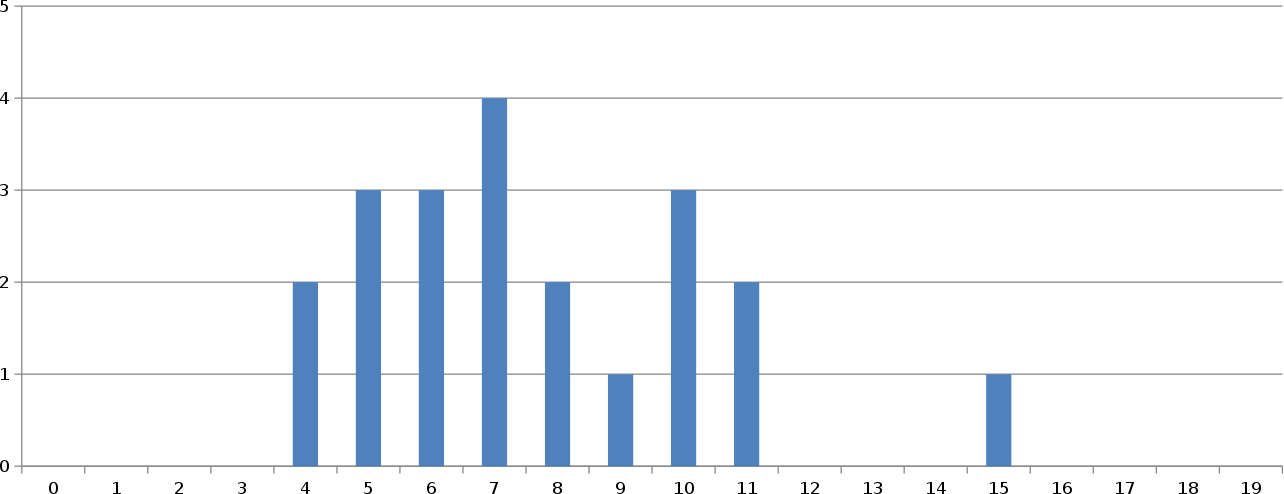
\includegraphics[width=.9\textwidth]{png/notes}
\end{center}

\end{document}

